\documentclass[runningheads]{llncs}

% ---------------------------------------------------------------
% Include basic ECCV package

% TODO REVIEW: Insert your submission number below by replacing '*****'
% TODO FINAL: Comment out the following line for the camera-ready version
%\usepackage[review,year=2026,ID=13008]{../ECCV_2026_Paper_Template/eccv}
\usepackage{eccv}
% TODO FINAL: Un-comment the following line for the camera-ready version
%\usepackage{../ECCV_2026_Paper_Template/eccv}

% Commonly used abbreviations (\eg, \ie, \etc, \cf, \etal, etc.)
\usepackage{eccvabbrv}

% The "axessiblity" package can be found at: https://ctan.org/pkg/axessibility?lang=en
\usepackage[accsupp]{axessibility}  % Improves PDF readability for those with disabilities.

% ---------------------------------------------------------------
% Other packages
\usepackage{amsmath}
\usepackage{amssymb}
\usepackage{bm}
\usepackage{graphicx}
\usepackage{booktabs}
\usepackage{multirow}
\usepackage{makecell}
\usepackage{array}
\usepackage{pifont}
\usepackage{tabularx}
\usepackage{subcaption}
\usepackage[table]{xcolor}
\usepackage{url}
\usepackage[utf8]{inputenc}
\usepackage{microtype}
\usepackage{tcolorbox}
\tcbuselibrary{breakable}
\usepackage{listings}

\usepackage{booktabs}   
\usepackage{graphicx}  
\usepackage{pifont}     
\usepackage{amssymb}
\newcommand{\cmark}{{\color{green!60!black}\ding{51}}} 
\newcommand{\xmark}{{\color{red!70!black}\ding{55}}} 
% Hyperref (recommended): load this late
\usepackage{hyperref}
\usepackage{colortbl}
\usepackage{xcolor}
\usepackage{orcidlink}


\newcommand{\hmark}{\textcolor{blue}{\sqrt{}\mkern-9mu{\smallsetminus}}}


\title{SciIR: A Large-scale Training Dataset and Benchmark for Scientific Image Reasoning Generation}
\titlerunning{SciIR}

\author{Zhiyuan Ma\inst{1}\orcidlink{0009-0006-3756-5621}\textsuperscript{*} \and
Zhengfeng Shi\inst{1}\textsuperscript{*} \and
Yuning An\inst{2} \and
Peize Li\inst{3} \and
Jiabao Wei\inst{4} \and
Ruijie Li\inst{5} \and
Junhao Xiao\inst{6} \and
Jianjun Li\inst{1}\orcidlink{0000-0002-5265-7624}\textsuperscript{\ensuremath{\dagger}} \and
Bowen Zhou\inst{7}}

\authorrunning{Z.~Ma et al.}

\institute{School of Computer Science and Technology, Huazhong University of Science and Technology, Wuhan, China\\
\email{jianjunli@hust.edu.cn}
\and
Department of Computer Science, Harbin Engineering University, Harbin, China
\and
King's College London, University of London, London, UK
\and
School of Computer Science and Technology, Beijing Institute of Technology, Beijing, China
\and
Department of Informatics, King's College London, London, UK
\and
School of Computer, Central China Normal University, Wuhan, China
\and
Department of Electronic Engineering, Tsinghua University, Beijing, China}



\newcolumntype{C}{>{\centering\arraybackslash}X}

\begin{document}
\maketitle

\begingroup
\renewcommand{\thefootnote}{}
\begin{NoHyper}
\footnotetext{* Equal contribution. \ensuremath{\dagger} Corresponding author.}
\end{NoHyper}
\endgroup
% Teaser figure: keep it above the abstract (non-floating)
% NOTE: caption's hypcap option is ignored for \captionof; disable it globally to avoid warnings.
\captionsetup{hypcap=false}
\begin{center}
    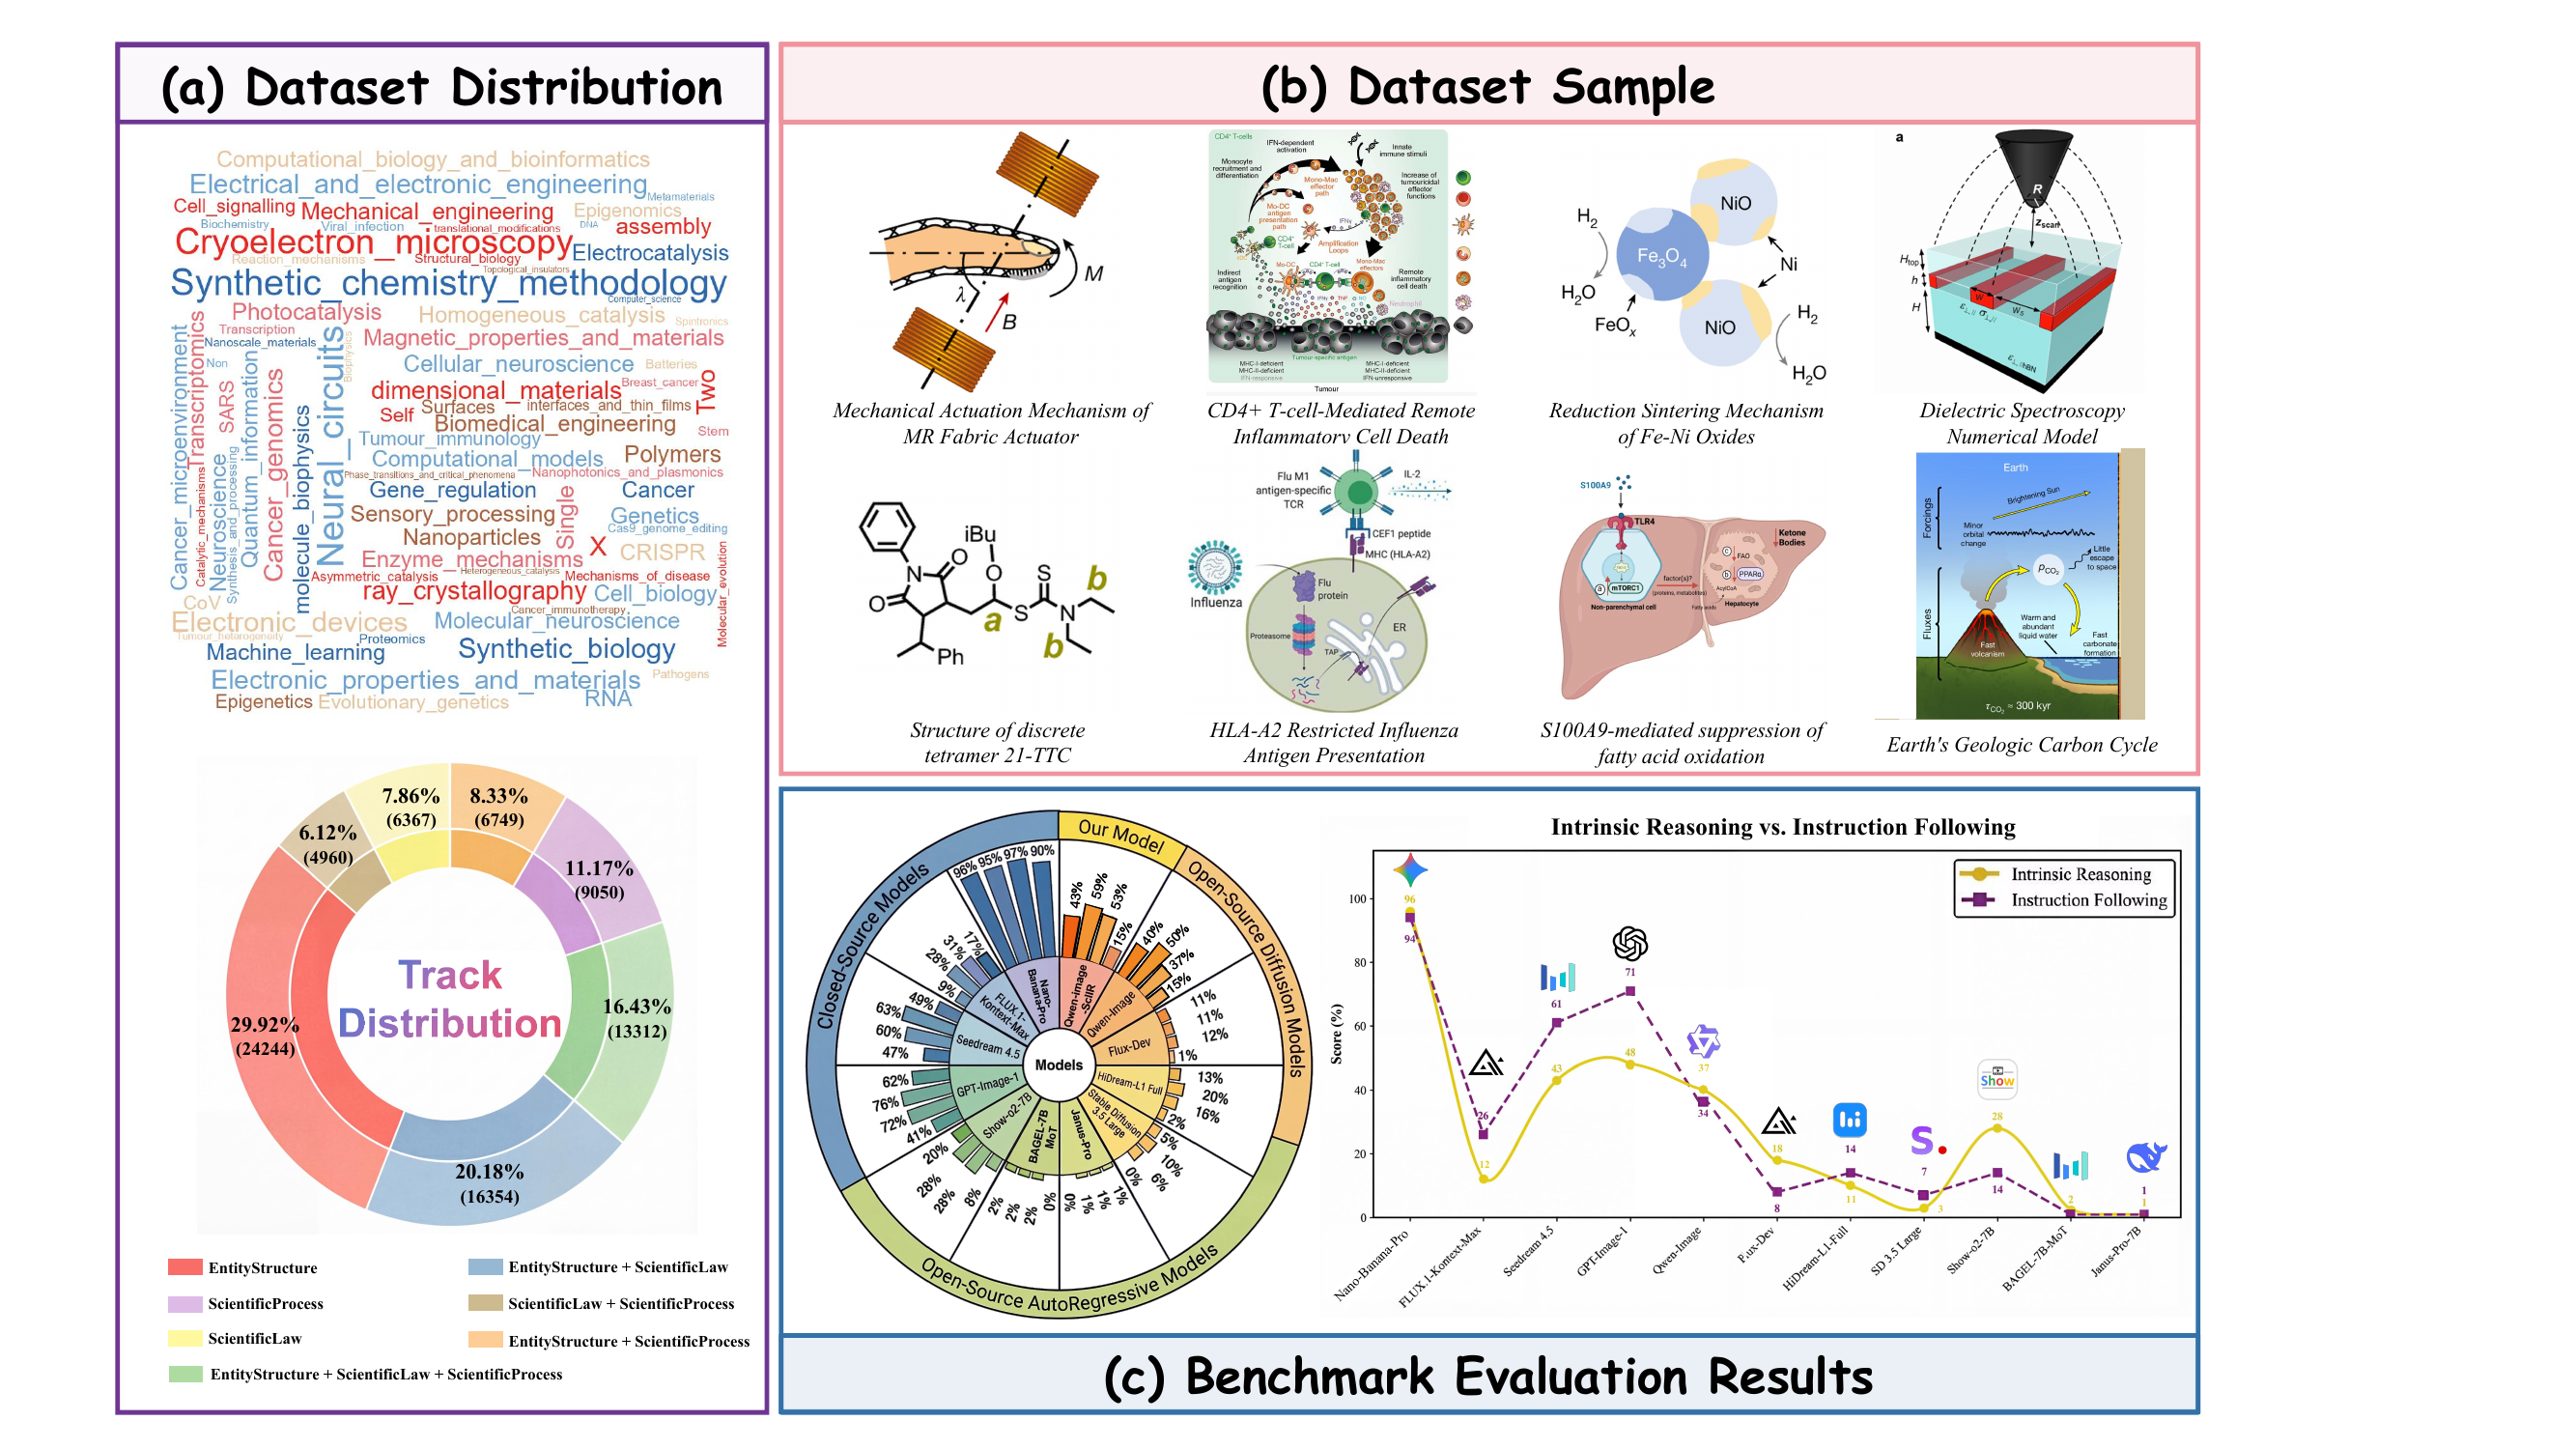
\includegraphics[width=\textwidth]{overview.pdf}
    \captionof{figure}{\textbf{Overview of SciIR.} (a) SciIR-82k: keyword word cloud and distribution across semiotic-oriented image generation tracks. (b) Example figures from diverse domains. (c) Illustration of SciIR-Bench results across various open- and closed-source models with a comparison of Intrinsic Reasoning vs. Instruction Following.}
    \label{fig:overview}
\end{center}

\begin{abstract}

While Text-to-Image (T2I) models have shown remarkable success in generating photorealistic visual content, they still struggle with the rigorous semantic alignment and logical reasoning required for scientific imagery.
Inspired by Peirce's Semiotic Triad, we introduce Scientific Image Reasoning (SciIR), a comprehensive resource for training and evaluation of scientific image generation.
We formalize scientific reasoning into three core dimensions: Entity Structure (\emph{Icon}), Scientific Process (\emph{Index}), and Scientific Law (\emph{Symbol}).
Specifically, to overcome the scarcity of training data in scientific image generation, we elaborately create SciIR-82k, a large-scale dataset containing over 80,000 high-quality scientific image-text pairs from cutting-edge publications.
The dataset is hierarchically organized according to the semiotic dimensions and incorporates a Scientific Reasoning Chain-of-Thought (Sci-RCoT) to explicitly model underlying visual logic.
For evaluation, we propose SciIR-Bench, which aligns with these three semiotic levels and employs an Atomic Checklist to convert the outcome-oriented scientific accuracy into process-oriented, verifiable, fine-grained questions.
Our extensive experiments reveal significant deficiencies in current models' scientific reasoning capabilities.
Furthermore, by fine-tuning on the SciIR-82k dataset, we developed the Qwen-Image-SciIR model, which achieves a substantial improvement on the SciIR-Bench, increasing the final score from 35\% to 43\%, laying a solid foundation for future advances in scientific image generation.Code is available at https://github.com/MAIR-Lab-HUST/SciIR

\keywords{Text-to-Image generation \and Scientific Image Reasoning }
\end{abstract}

% In recent years, advances in Text-to-Image (T2I) generation have produced high-quality models across various architectures. Diffusion-based models~\cite{yang2023improving,esser2024scaling,gao2024lumina,xie2025sana,qin2025lumina} have demonstrated impressive capabilities in visual realism and stylistic diversity. Meanwhile, autoregressive (AR) models~\cite{sun2024autoregressive,zhang2024var,wang2024emu3,chen2025janus} have further extended the boundaries of semantic alignment and instruction following. More recently, reasoning-augmented approaches have begun to incorporate chain-of-thought (CoT) strategies~\cite{liao2025imagegen} to handle complex prompts. These developments have democratized content creation, allowing users to generate complex artistic scenes with simple text prompts. However, despite excelling in open-domain creativity, these models still face a critical bottleneck in performing rigorous reasoning within complex, constraint-heavy scenarios.

\section{Introduction}
Recent advances in Text-to-Image (T2I) generation have yielded high-quality models: diffusion-based approaches \cite{yang2023improving,esser2024scaling,gao2024lumina,xie2025sana,qin2025lumina,ma2025efficient,ma2024neural} deliver exceptional visual realism and stylistic diversity, autoregressive methods \cite{sun2024autoregressive,zhang2024var,wang2024emu3,chen2025janus} excel at semantic alignment and complex instruction following, and emerging reasoning-augmented techniques integrate chain-of-thought (CoT) strategies \cite{liao2025imagegen,pan2025self} to help resolve ambiguities and map abstract concepts to concrete visual attributes. Despite these gains, T2I models remain fundamentally constrained when required to perform rigorous reasoning under complex, multi-constraint scenarios—most notably in scientific imagery, which must strictly adhere to physical laws, accurate topology, and causal logic. Even state-of-the-art closed-source systems (\eg, \texttt{Nano-Banana}) that achieve high perceptual fidelity and object-level consistency frequently violate domain-specific logical constraints, producing results that are ``visually plausible but factually incorrect''.

By contrast, open-source alternatives \cite{esser2024scaling,xie2024show,deng2025emerging,labs2025flux,wu2025qwen,cai2025hidream,ma2025janusflow} face more fundamental challenges: in knowledge-intensive contexts, they often struggle to internalize domain-specific knowledge and satisfy strict scientific constraints.
This divergence underscores a vital principle: \textit{Perceptual fidelity does not equate to reasoning robustness, and visual polish cannot compensate for the absence of scientific validity.}
These methodological gaps crystallize into three bottlenecks that impede scientific image generation:

\begin{enumerate}
  \item \textit{Data aspect — scarcity of logic-annotated resources.} High-quality scientific figures with explicit reasoning annotations are scarce because producing and annotating them requires deep, domain-specific expertise. Existing datasets therefore lack the ``visual logic'' necessary for models to learn the dependencies required to map text into scientifically accurate structures.
  \item \textit{Evaluation aspect — lack of scientific-correctness standards.} Current evaluation frameworks leave a structural gap in assessing scientific correctness. Although recent tools such as AutoFigure~\cite{zhu2026autofigure} and PaperBanana~\cite{zhu2026paperbanana} facilitate automated figure generation, their evaluation emphasizes layout and workflow rather than underlying scientific logic. Moreover, benchmarks (e.g., SridBench~\cite{chang2025sridbench}) often do not offer fine-grained semantic diagnosis, making it hard to define a verifiable ground truth for auditing the multidimensional constraints in scientific imagery.
  \item \textit{Model aspect — deficiencies in enforcing scientific constraints.} Open-source models in particular lack specialized scientific reasoning and therefore struggle to satisfy hard constraints such as topology or reaction causality, frequently producing hallucinations that violate basic physical laws.
\end{enumerate}

Motivated by the above three aspects, we propose \textbf{SciIR}, a semiotic triad-based dataset and benchmark designed to promote scientific rigor in image reasoning generation. 
In short, our main contributions are summarized as follows:
\begin{itemize}
  \item We construct \textbf{SciIR-82k}, a large-scale refined dataset of over $80,000$ scientific image-text pairs from \textit{Nature} and \textit{Nature Communications}. This dataset is enhanced with Sci-RCoT annotations, which explicitly formalize latent visual reasoning pathways to train models on underlying scientific logic.
  \item We introduce \textbf{SciIR-Bench}, the first benchmark to systematically categorize evaluation tracks based on multidimensional scientific correctness, employing a novel atomic checklist to provide fine-grained, verifiable questions.
  \item We develop \textbf{Qwen-Image-SciIR}, a strong open-source baseline that boosts the final score on SciIR-Bench from $35\%$ to $43\%$ by fine-tuning Qwen-Image-2512 on SciIR-82k, and serves as a reliable starting point for future research on scientific image reasoning generation.
\end{itemize}

% \textbf{(1)SciIR-82k Dataset:} We build a large-scale, high-fidelity dataset comprising over 80,000 scientific image-text pairs curated from top-tier literature. Crucially, we augment this data with Scientific Reasoning Chain-of-Thought (Sci-RCoT), transforming implicit visual information into explicit reasoning paths to train models on the logic behind the pixels.

% \textbf{(2)SciIR-Bench with Atomic Checklist:} We propose a rigorous evaluation suite that decomposes scientific correctness into verifiable atomic constraints. This novel protocol achieves high correlation with human expert judgment (Pearson’s r = 0.792), significantly outperforming traditional metrics such as CLIPScore.

% \textbf{(3)Proven Effectiveness via Fine-tuning:} We conduct extensive experiments on 11 state-of-the-art models, revealing substantial performance disparities between closed-source and open-source systems. Furthermore, we demonstrate that fine-tuning an open-source model (Qwen-Image) on the SciIR-82k dataset yields significant improvements, boosting overall scientific accuracy from 25\% to 37\% and underscoring the critical value of reasoning-aligned data.


\section{Related Work}
\begin{table}[t]
\caption{Comparison of SciIR-82k with representative T2I datasets.}
\label{tab:t2i_dataset_comparison}
\centering
\small
\setlength{\tabcolsep}{3pt}
\begin{tabular}{lccc}
\toprule
\textbf{Dataset} & \textbf{Scale} & \textbf{Text Length} & \textbf{Reasoning Type} \\
\hline
\rowcolor{gray!15} \multicolumn{4}{c}{\textit{\textbf{Synthetic Image Datasets}}} \\
JourneyDB\cite{sun2023journeydb} & 4M & Short & None \\
PixelProse\cite{pixelprose24} & 16M & Long & None \\
FLUX-Reason-6M\cite{fang2025flux} & 6M & Short & Visual \\
Science-T2I\cite{li2025science} & 20K & Short & Outcome-oriented \\
\midrule
\rowcolor{gray!15} \multicolumn{4}{c}{\textit{\textbf{Non-Synthetic Image Datasets}}} \\
CC-12M\cite{changpinyo2021cc12m} & 12M & Short & None \\
LAION-Aesthetics\cite{schuhmann2022laion} & 120M & Short & None \\
TextCaps\cite{sidorov2020textcaps} & 28K & Short & None \\
DOCCI\cite{OnoeDocci2024} & 15K & Long & None \\
\textbf{SciIR-82k (Ours)} & \textbf{82K} & \textbf{Short + Long} & \textbf{ Process-oriented} \\
\bottomrule
\end{tabular}
\end{table}

\subsection{Text-to-Image Datasets}

Current text-to-image (T2I) datasets generally lack the cognitive depth required for complex scientific synthesis. As shown in \cref{tab:t2i_dataset_comparison}, both synthetic and non-synthetic collections provide predominantly descriptive captions, omitting explicit reasoning chains or structured semantic relations. Specifically, while synthetic datasets \cite{sun2023journeydb,pixelprose24,fang2025flux,li2025science} provide large-scale, controllable supervision, they often inherit biases from source models—prioritizing visual plausibility and stylistic diversity over rigorous logical consistency. Conversely, non-synthetic datasets \cite{sidorov2020textcaps,changpinyo2021cc12m,OnoeDocci2024,schuhmann2022laion} source web image-text pairs to cover everyday concepts, but their typically short captions lack domain knowledge and explicit logical structures.
While scientific datasets like Science-T2I \cite{li2025science} leverage specialized knowledge to mitigate inconsistencies in generated diagrams, such early efforts remain limited in scale and prioritize final visual correctness. Consequently, their reliance on post-hoc preference modeling for implicit, outcome-oriented reasoning fails to support the intrinsic, process-oriented reasoning required during generation.
To bridge this gap, we introduce SciIR-82k. Sourced from academic publications, it is enriched with detailed Sci-RCoT annotations that formalize the logical steps for figure construction. By explicitly addressing complex scientific logic spanning Structure, Process, and Law—capturing structural relationships, causal mechanisms, and scientific principles—SciIR-82k provides process-oriented supervision. This explicit formalization allows models to learn rigorous, reasoning-conditioned visualizations from scratch, grasping not merely how scientific images look, but the underlying rationale behind their structured representations.

\begin{table}[tb]  
\caption{Comparison of SciIR-Bench with representative T2I benchmarks. \textbf{SL}: Scientific Law, \textbf{ES}: Entity Structure, \textbf{SP}: Scientific Process.}
\label{tab:sciir_comparison}
\centering
\scriptsize  
\setlength{\tabcolsep}{3pt} 
\renewcommand{\arraystretch}{1.1} 
\begin{tabular}{lllccccc} 
\toprule
\multirow{2}{*}{\textbf{Benchmark}} & \multirow{2}{*}{\textbf{Scale}} & \multirow{2}{*}{\textbf{Domain}} & \multicolumn{4}{c}{\textbf{Evaluation Dimensions}} & \multirow{2}{*}{\textbf{\shortstack{Fine-grained}}} 
\\ \cmidrule(lr){4-7}
& & & \makebox[0.9cm][c]{\textbf{SL}} & \makebox[0.9cm][c]{\textbf{ES}} & \makebox[0.9cm][c]{\textbf{SP}} & \makebox[0.9cm][c]{\textbf{Text}} & 
\\
\midrule
GenEval++\cite{ye2025echo}       & 280    & Generic      & \xmark & \cmark & \xmark & \xmark & \cmark \\
T2I-CompBench\cite{huang2023t2i}   & 6k  & Generic      & \xmark & \cmark & \xmark & \xmark & \cmark \\
WISE\cite{niu2025wise}             & 1k    & Generic      & \cmark & \xmark & \cmark & \xmark & \xmark \\
R2I-Bench\cite{chen2025r2i}        & 3068   & Generic      & \xmark & \xmark & \cmark & \xmark & \cmark \\
T2I-ReasonBench\cite{sun2025t2i} & 800  & Generic      & \cmark & \cmark & \xmark & \xmark & \cmark \\
ScImage\cite{zhang2024scimage}         & --   & Method. Diags.& \xmark & \cmark & \xmark & \cmark & \xmark \\
PaperBananaBench\cite{zhu2026paperbanana}& 292   & Method. Diags.& \xmark & \cmark & \cmark & \cmark & \xmark \\
FigureBench\cite{zhu2026autofigure}     & 3300   & Method. Diags.& \xmark & \cmark & \cmark & \cmark & \xmark \\
SridBench\cite{chang2025sridbench}       & 1120   & Sci. Illus.  & \cmark & \cmark & \xmark & \cmark & \xmark \\
SciGenBench\cite{lin2026scientific}     & --    & Sci. Illus.& \cmark & \cmark & \xmark & \cmark & \cmark \\
\midrule
\textbf{SciIR-Bench (Ours)} & \textbf{800} & \textbf{Sci. Illus.} & \textbf{\cmark} & \textbf{\cmark} & \textbf{\cmark} & \textbf{\cmark} & \textbf{\cmark} \\ 
\bottomrule
\end{tabular}
\end{table}

\subsection{Text-to-Image Benchmark}
Existing benchmarks evaluate generation through three evolving perspectives. \textit{1) Perceptual Quality:} Early metrics like IS \cite{salimans2016improved} and FID \cite{heusel2017gans} assess distributional realism. \textit{2) Prompt Alignment:} Benchmarks such as T2I-CompBench \cite{huang2023t2i} and GenEval++ \cite{ye2025echo} quantify textual fidelity via VLM-based scoring \cite{hessel2021clipscore, ghosh2023geneval, hu2023tifa}. \textit{3) Semantic Plausibility:} Recent frameworks (\eg, WISE \cite{niu2025wise}, T2I-ReasonBench \cite{sun2025t2i}) target logical reasoning using LLMs. Within the domain of scientific figure generation, PaperBananaBench \cite{zhu2026paperbanana} and FigureBench \cite{zhu2026autofigure} concentrate on the evaluation of flowcharts and statistical diagrams. While SridBench \cite{chang2025sridbench} specifically targets scientific diagrams, it remains focused on broad interpretation rather than fine-grained generative constraints.

To address this structural opacity, we posit that scientific correctness cannot be treated as a monolithic metric but requires systematic decomposition. Drawing inspiration from Peirce's Semiotic Triad \cite{peirce1931collected}, we decompose scientific correctness into \textit{law}, \textit{structure}, and \textit{process}. However, we observe that no existing benchmark comprehensively covers all three dimensions (as shown in \cref{tab:sciir_comparison}), failing to diagnose specific atomic violations (\eg, broken causal links). To bridge this gap, we propose SciIR-Bench, a diagnostic framework that holistically assesses these dimensions through explicit, verifiable criteria.

\subsection{Methods for Scientific Image Generation}
Recent research has also advanced the automated generation of scientific illustrations. For example, AutoFigure\cite{zhu2026autofigure} focuses on producing publication-ready illustrations from long-form text, emphasizing layout and aesthetics, while PaperBanana specializes in automating and improving the visualization quality of methodological workflows \cite{zhu2026paperbanana}. Alternatively, ImgCoder\cite{lin2026scientific} prioritizes programmatic synthesis (code generation) to circumvent pixel-level reasoning challenges, though it lacks the visual expressivity required for rendering nuanced or complex graphic details. Despite these advances, such efforts remain primarily confined to procedural and architectural diagrams. In contrast, our work targets scientific schematics that encode underlying natural principles (\eg, physical laws and causal mechanisms). Moving beyond layout fidelity, we explicitly model and evaluate \emph{scientific correctness}, requiring models not only to reproduce structural relationships but also to internalize and faithfully represent the domain-specific principles governing the depicted phenomena.

\section{SciIR-82k Dataset}
To systematically evaluate the scientific reasoning abilities of T2I models, we introduce SciIR-82k, a large-scale dataset of over $80,000$ high-quality scientific image-text pairs with complete annotations. As shown in \cref{fig:wide-example}, our SciIR-82k is grounded in a semiotic triad and constructed through a multi-stage automated pipeline for promoting scientific fidelity.  

\subsection{Theoretical Taxonomy: Semiotic Triad}
\label{sec:Semiotic Triad}

Scientific images are not merely visual imagery but abstract structures encoding logical relations and physical constraints.
To effectively formalize these, we ground our dataset in Peirce's Semiotic Triad~\cite{peirce1931collected}, \ie, \textit{Icon}, \textit{Index}, and \textit{Symbol}, which respectively correspond to the cognitive layers for scientific reasoning: \textit{1) Entity Structure} corresponds to \textit{iconic} representation via topological fidelity, which evaluates the geometric hierarchical reconstruction and spatial alignment of scientific entities.
\textit{2) Scientific Process} corresponds to \textit{indexical} representation indicating causal or temporal correlations, involving state transitions, experimental workflows, or causal chains.
\textit{3) Scientific Law} corresponds to \textit{symbolic} representation governed by abstract rules, ensuring adherence to fundamental laws (\eg, conservation of energy, molecular valence).
This taxonomy transcends simple visual-text alignment, establishing a structured framework for deep scientific reasoning.

\subsection{Corpus Construction}

Our corpus comprises articles licensed under CC BY 4.0 from \textit{Nature} and \textit{Nature Communications} to ensure authority; comprehensive compliance and provenance details are outlined in Appendix A.
From about $360$k raw figures, we employ Ultralytics-YOLO11 \cite{jocher2024ultralytics} as an automated layout analyzer to decompose multi-panel figures into semantically independent subfigures, which are then standardized to a $1024\times1024$ resolution.
Afterwards, a two-stage filtering pipeline---VLM-based screening with InternVL3.5 \cite{wang2025internvl3} to retain corresponding schematics, followed by manual verification---finally extracts over $80$k high-quality subfigures and their corresponding captions and content.
Data processing details are provided in the Appendix B.

\subsection{Semiotic Stratification}


We implement a stratification strategy to align the raw data with our semiotic taxonomy (\cref{sec:Semiotic Triad}).
Using Qwen3-VL \cite{Qwen3-VL} as a domain-specific evaluator, we assess each sample’s relevance score $s\in[1,10]$ to the three reasoning tracks (\texttt{Entity Structure}, \texttt{Scientific Process}, or \texttt{Scientific Law} ).
This categorization serves as a routing mechanism, directing images to targeted annotation pipelines according to their dominant semiotic attributes.

\begin{figure*}[t]
    \centering
    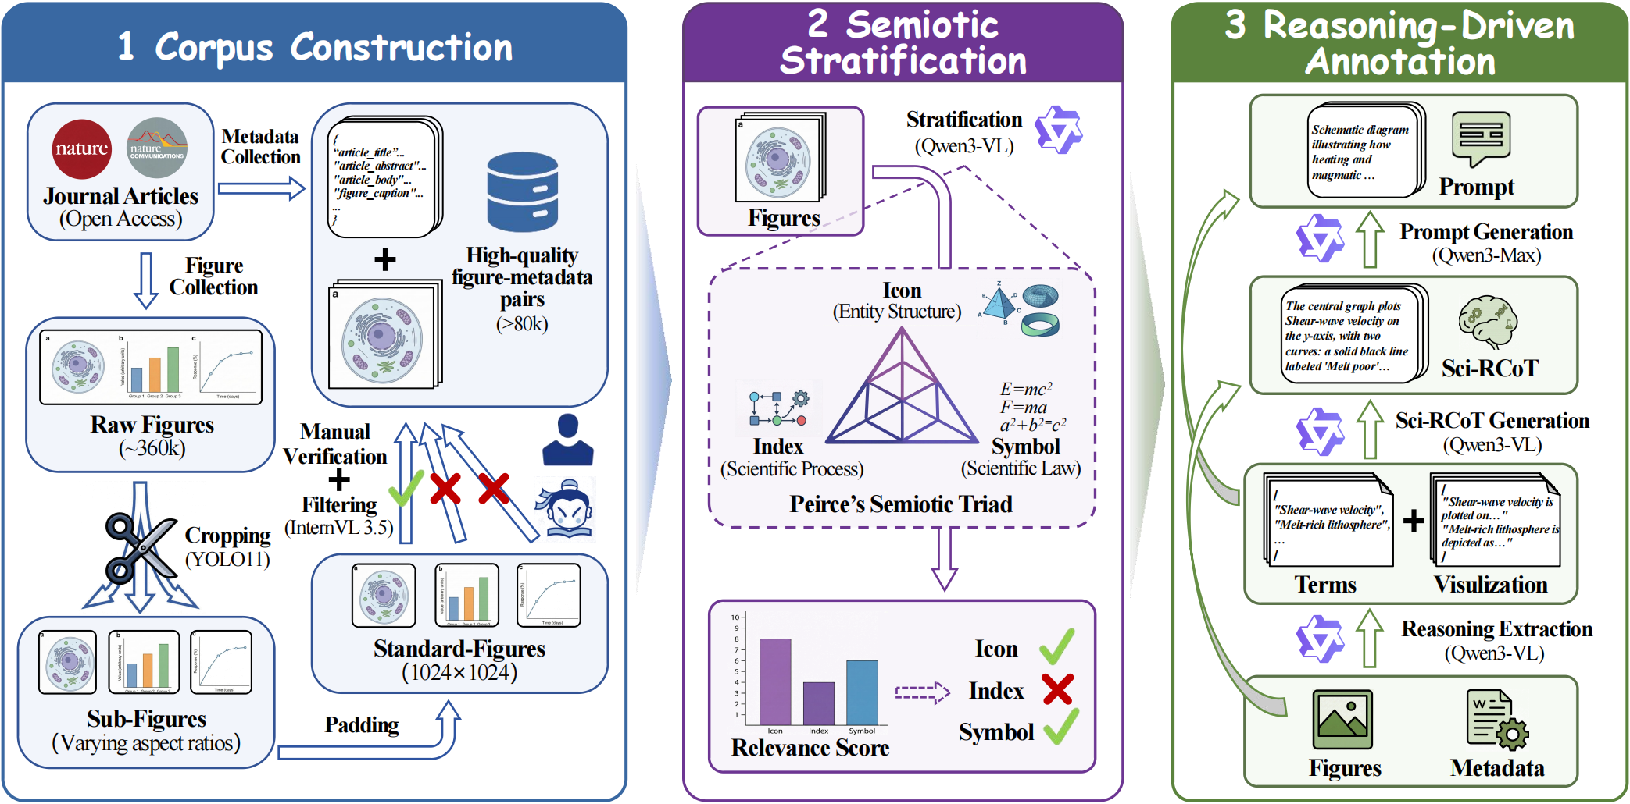
\includegraphics[width=\textwidth]{dataset.pdf}
\caption{\textbf{Overview of the SciIR-82k pipeline grounded in Peirce’s Semiotic Triad\cite{peirce1931collected}.} The framework comprises three stages: (1) Corpus Construction, employing YOLO11 and InternVL 3.5 for sub-figure extraction and filtering; (2) Semiotic Stratification, categorizing samples into Icon, Index, and Symbol tracks; and (3) Reasoning-Driven Annotation, which leverages Qwen3 models to reverse-engineer Sci-RCoT and prompts.}
    \label{fig:wide-example}
\end{figure*}

\subsection{Reasoning-Driven Annotation}
\label{sec:semiotic_pipeline}

%Standard generative paradigms typically follow a forward trajectory: Abstract Prompt $\rightarrow$ Logical Deduction $\rightarrow$ Visual Output.
In contemporary text-to-image and multimodal generation frameworks, the process typically follows a forward pipeline: Abstract Prompt $\rightarrow$ Logical Deduction $\rightarrow$ Visual Output, where high-level semantic intent is progressively instantiated into concrete visual representations.
For high-fidelity reasoning annotation, we invert this chain via \textit{logical reverse engineering}: reconstructing latent scientific reasoning (\ie, Sci-RCoT) from ground-truth images to derive precise prompts, with Qwen3-VL \cite{Qwen3-VL} for visual grounding and Qwen3-Max \cite{qwen3} for semantic abstraction.

\textbf{Taxonomy-Driven Reasoning Extraction.} In the first phase, Qwen3-VL \cite{Qwen3-VL} extracts taxonomy-guided structured information, prioritizing visual evidence (Image $>$ Caption $>$ Text).
The model parses input into JSON, decoupling: \textit{1) Terms:} Image-validated entities and nomenclatures. \textit{2) Visualization:} Descriptions of visual grounding (\eg, geometry, layout).
This taxonomy-driven extraction enforces semantic decomposition of scientific content, reduces hallucination, and converts free-form multimodal understanding into controllable, fine-grained reasoning units suitable for downstream transformation.

\textbf{Sci-RCoT Generation.} Afterwards, Qwen3-VL \cite{Qwen3-VL} synthesizes a Scientific Reasoning CoT (Sci-RCoT) by re-examining the image to integrate visual style (\eg, schematic diagrams) and text rendering requirements with ``Visualization'' entries.
 By transforming discrete reasoning units into a continuous visual reconstruction process, Sci-RCoT, as an explicit reasoning trace, bridges symbolic reasoning and holistic scene composition,  elucidating the causal logic underlying the mapping of abstract concepts to concrete spatial arrangements.

\textbf{Prompt Generation.} Eventually, Qwen3-Max \cite{qwen3} distills Sci-RCoT into a concise prompt via a ``Term-Substitution'' strategy: Visualization descriptions are replaced with canonical scientific terms while preserving the original visual style as the leading phrase, and only explicitly required textual renderings are retained. This produces a 
synchronized pair of abstract prompt and retained text. This step removes redundant visual detail while preserving scientific semantics, yielding a compact yet information-complete prompt representation. The resulting abstraction enhances controllability, improves semantic consistency across samples, and provides high-quality structured supervision for process reasoning-aware image generation and evaluation.

Overall, this pipeline performs logical reverse engineering from images to prompts by progressively transforming visual evidence into structured reasoning traces and finally into compact prompt representations. This design enforces explicit alignment between image structures, textual elements, and reasoning units, producing controllable and logically grounded prompts. The resulting annotations provide reliable supervision for evaluating and training process reasoning-aware scientific image generation models.
%过程感知的
\section{SciIR-Bench}
\begin{figure*}[t]
    \centering
    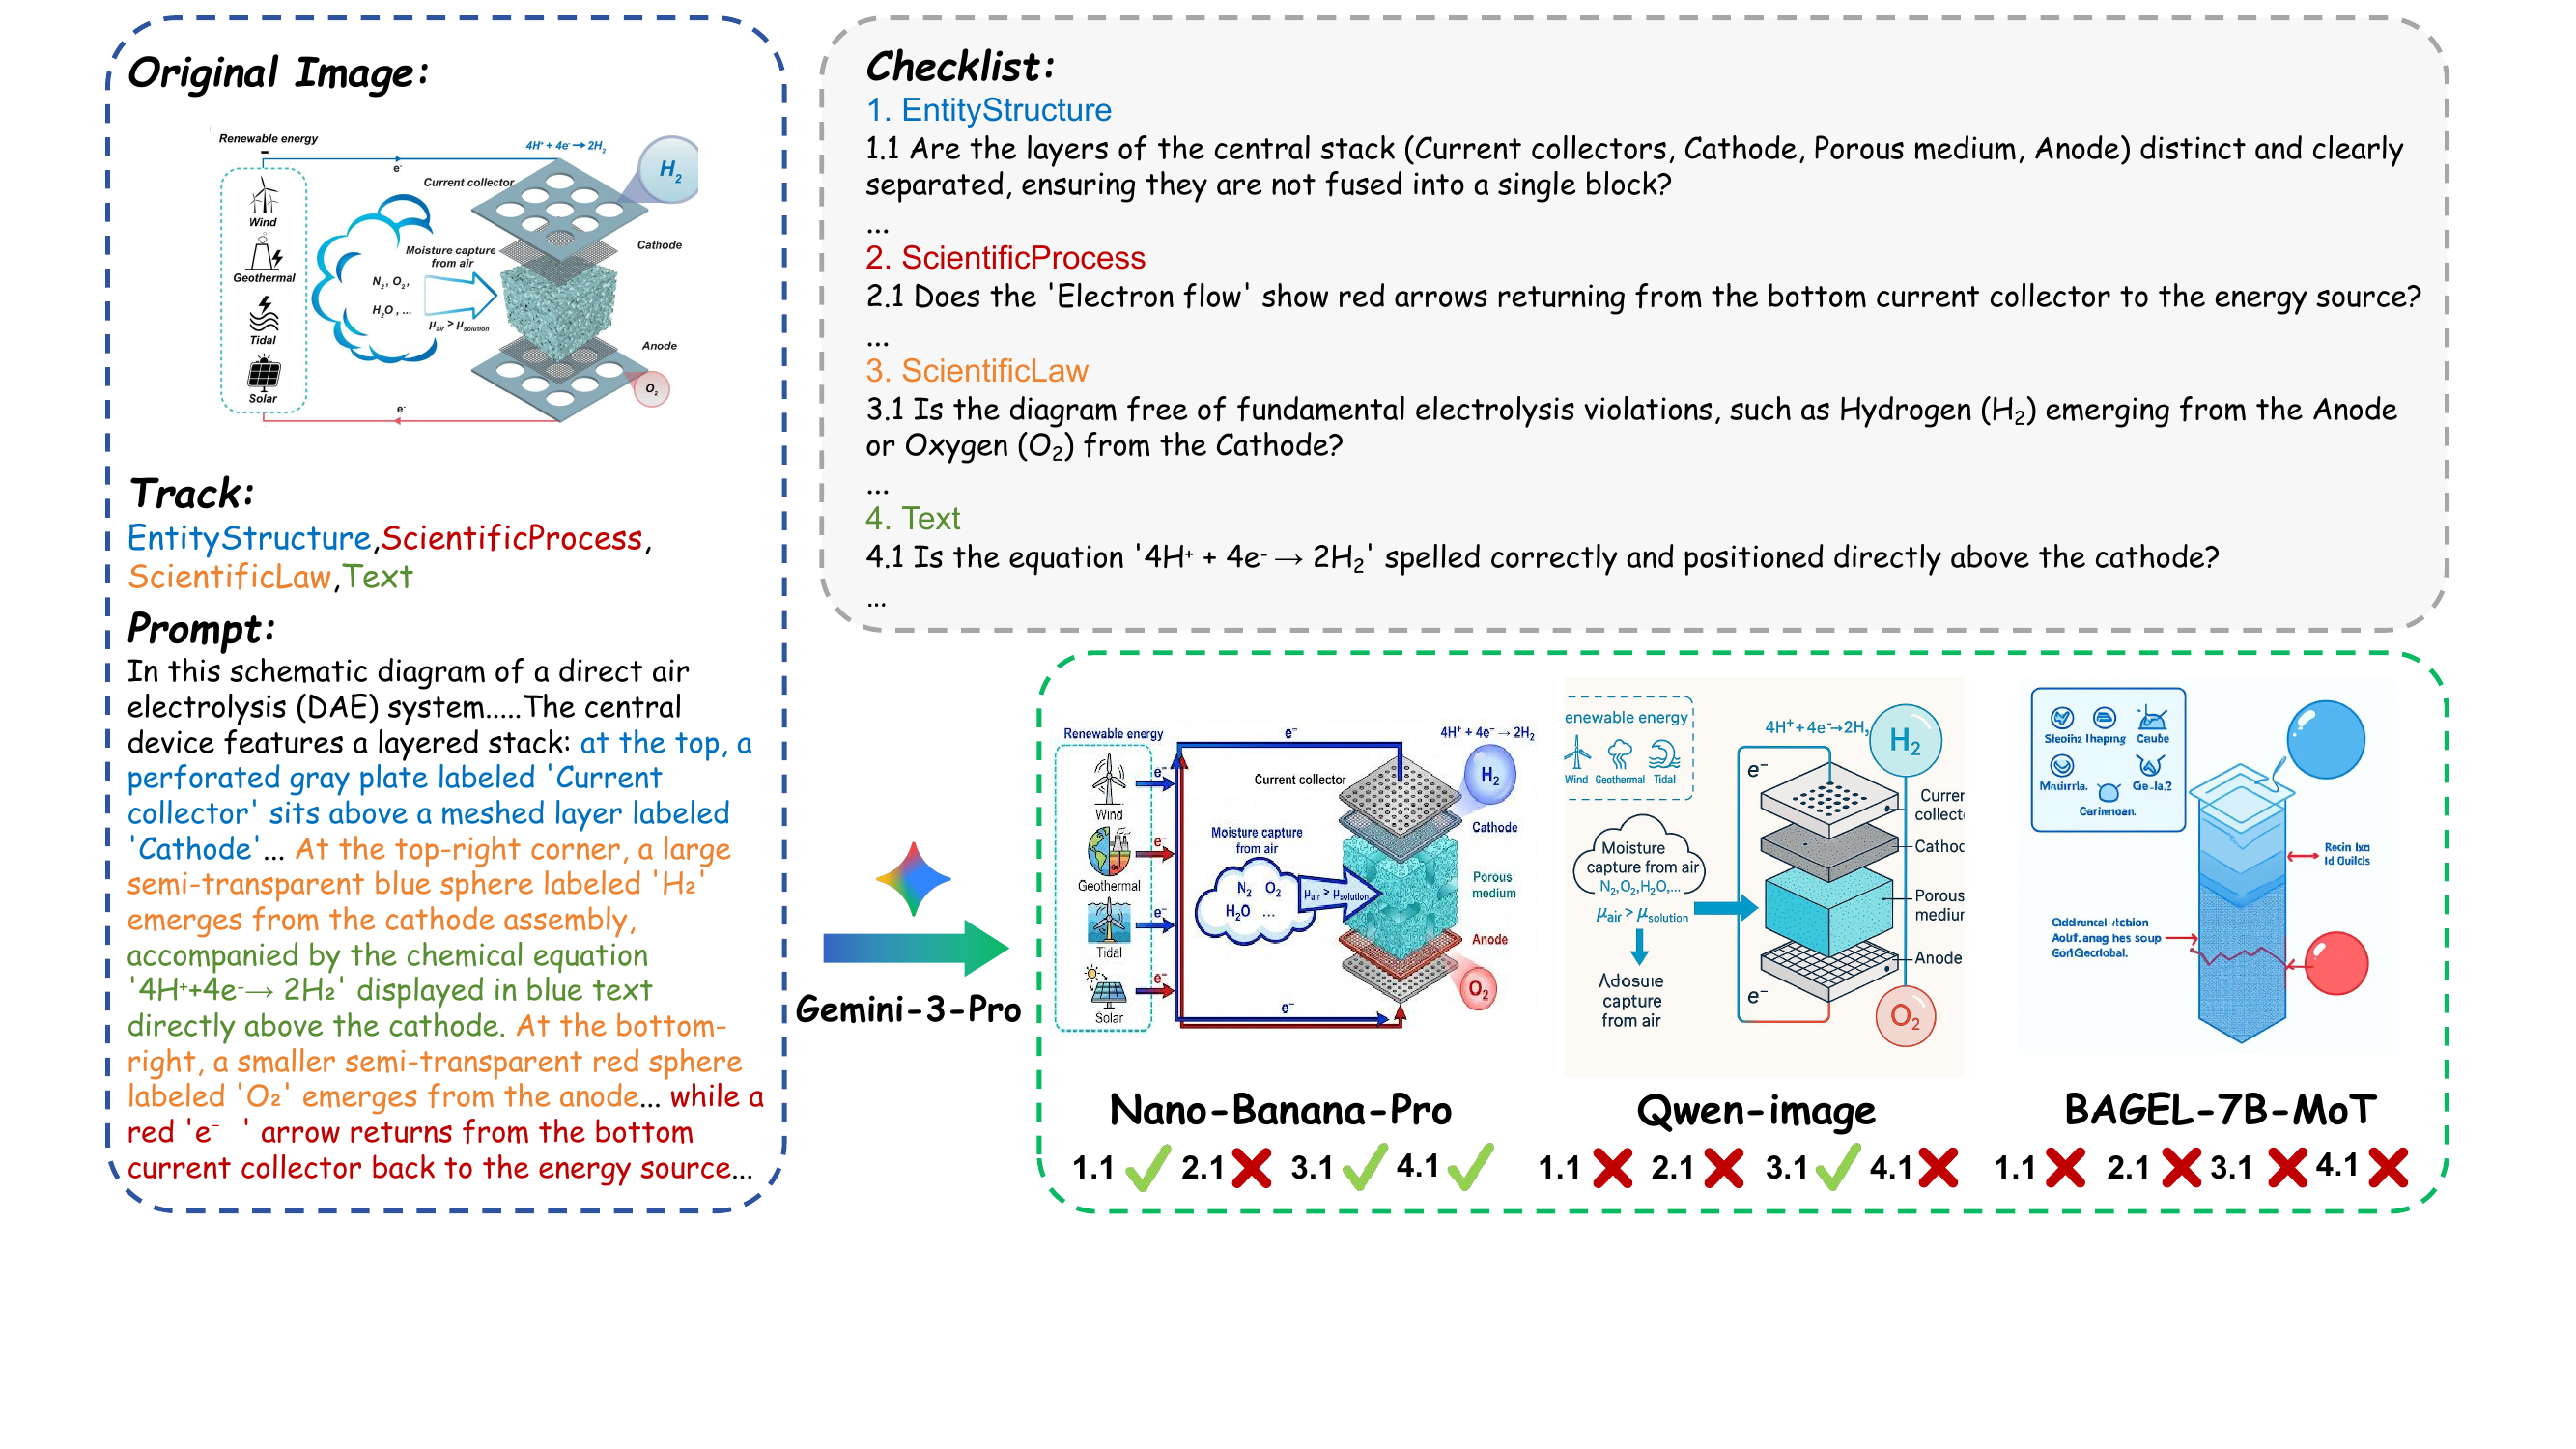
\includegraphics[width=\textwidth]{benchmark.pdf}
    \caption{\textbf{An evaluation instance from SciIR-Bench.} Prompt from a sample covering all four tracks is used to guide various models in generating images. The output is then scrutinized by Gemini-3-Pro using a dimension-specific atomic checklist.}
    \label{fig:wide-example1}
\end{figure*}

To systematically evaluate the scientific reasoning and generation capabilities of current text-to-image models, we develop the SciIR-Bench (\cref{fig:wide-example1}). This benchmark moves beyond traditional holistic image quality metrics and instead measures whether models can faithfully instantiate structured scientific content—such as correctly rendering labeled entities, preserving spatial and topological relations, and accurately depicting multi-stage processes—without introducing unsupported elements or logical contradictions in the visualization.
%具体化

%什么的样例
\subsection{Evaluation Benchmark}

\textbf{Candidate Selection and Filtration.} From the massive corpus of processed samples, we distilled a high-quality evaluation benchmark consisting of 800 test instances. To ensure the benchmark challenges the upper limits of current models, we enforced a rigorous protocol focusing on both the breadth of scientific domains and the depth of reasoning complexity. We prioritized samples exhibiting High Term Density (term count $>3$) to guarantee sufficient semantic content. Details of the screening process are provided in the Appendix C. Furthermore, to verify multimodal reasoning capabilities, we selected candidates that necessitate compound reasoning across our theoretical dimensions, filtering out samples that do not contain valid reasoning paths in at least two of the three semiotic tracks (\texttt{Entity Structure}, \texttt{Scientific Process}, or \texttt{Scientific Law}).

\textbf{Taxonomy-Based Grouping.} To systematically evaluate model performance across different reasoning intersections, we exploit a four-folds strategy to categorize the filtered candidates into four distinct evaluation groups ($N=200$ per group). The first group represents the most complex ``holistic'' reasoning scenario, containing samples that simultaneously encompass attributes of all three tracks: Scientific Law, Entity Structure, and Scientific Process. The remaining three groups are constructed to test pairwise reasoning capabilities, covering the specific intersections of Law-Entity, Law-Process, and Entity-Process, respectively. This combinatorial approach ensures that the benchmark evaluates not just isolated knowledge but the model’s ability to synthesize conflicting constraints from multiple semiotic dimensions.
%需要例子

\textbf{Adaptive Difficulty Stratification.} Within each group, we bifurcated samples into two difficulty levels based on scientific term density to strictly disentangle \textit{Instruction Following} from \textit{intrinsic reasoning}:
\textit{1) Instruction Following (IF).}
Samples with high term density ($>$ median) are paired with the detailed Sci-RCoT. For these semantically saturated images, compressing the input into a concise prompt inevitably leads to \textit{semantic erosion}, causing the model to omit critical scientific details. By providing the exhaustive Sci-RCoT, we eliminate the ambiguity space, thereby strictly testing the model's fidelity in visualizing complex, fine-grained instructions.
\textit{2) Intrinsic Reasoning (IR).}
Conversely, samples with lower term density are paired with the abstract Prompt. In this regime, the input provides only high-level nomenclature without visual cues. This information sparsity compels the model to bridge the gap using latent domain knowledge, effectively evaluating its capacity to autonomously reason out valid spatial layouts and causal logic from abstract concepts.

\subsection{Evaluation Metrics}
\label{sec:metric}
Traditional generative metrics such as FID\cite{heusel2017gans} or CLIPScore\cite{radford2021learning} focus primarily on image fidelity or broad semantic similarity. However, these metrics fail to capture the factual correctness and logical consistency essential for scientific modeling. To bridge this gap, we propose a fine-grained, interpretable evaluation protocol designed to mimic the rigor of human peer review. Unlike black-box scoring, this VLM-driven checklist operationalizes evaluation through a transparent, three-stage automated pipeline comprising ground truth extraction, atomic questioning, and evidence-based refereeing.

\textbf{Atomic Checklist Generation.} We utilize the structured Reasoning content (extracted in Phase 1) as the absolute ground truth, avoiding reliance on potentially noisy reference images. To ensure comprehensive coverage, the checklist generation is strictly term-driven: for every ``Scientific Term'' identified in the reasoning structure, a VLM (\texttt{Gemini-3-Pro}) generates a corresponding binary validation query. This enforces Atomicity, as each question is strictly scoped to verify the visual manifestation of a single semantic unit (\eg, the specific morphology of a protein or the directionality of a process arrow). Moreover, to address the issue of hallucination, we generate supplementary adversarial questions tailored to each specific track to explicitly probe for domain-specific fabrications (\eg, non-existent chemical bonds), ensuring the model is penalized for inventing scientifically invalid details.

\textbf{Automated Evaluation.} In the adjudication phase, an advanced VLM acts as a ``Senior Scientific Reviewer'' to evaluate the generated images against the checklist. To prevent hallucinated judgments, we enforce a Visual Evidence Retrieval protocol: the referee must explicitly locate and describe the specific visual element mentioned in the query before assigning a verdict. The evaluation logic is strictly compartmentalized by category—Text is judged on spelling and positional exactness, while scientific tracks (\texttt{Entity Structure}, \texttt{Scientific Process}, \texttt{Scientific Law}) are evaluated on topological and causal logic. This separation ensures graphical errors result in scientific penalties, while textual errors are isolated to the text score.

\textbf{Accuracy Score.} Distinct from standard metrics that average accuracy across all questions, we adopt a rigorous sample-level pass rate to reflect the intolerance for error in scientific communication. Formally, let $Q_{i,c}$ be the set of atomic questions generated for a sample $i$ within a specific reasoning category $c$ (\eg, \texttt{Scientific Process}), and let $s(q) \in \{0,1\}$ denote the binary score of a single question $q$. The validity of a sample $i$ in category $c$, denoted as $V_{i,c}$, is defined by a strict veto mechanism:

\begin{equation}
V_{i,c} = \begin{cases} 
1 & \text{if } \prod_{q \in Q_{i,c}} s(q) = 1 \\
0 & \text{otherwise}
\end{cases}
\end{equation}

A sample is considered valid for a specific track only if it passes every atomic check associated with that track; a single failure renders the sample scientifically compromised for that dimension. The final accuracy score for category $c$ is calculated as the percentage of valid samples across the dataset $D$:

\begin{equation}
\text{Accuracy Score}_{c} = \frac{1}{|D|} \sum_{i \in D} V_{i,c}
\end{equation}

This strict metric provides a granular and uncompromising diagnostic of model performance, ensuring that high scores reflect true scientific robustness rather than partial hallucinatory success.
\begin{table}[t]
\caption{\textbf{Evaluation on SciIR-Bench.} We report the Accuracy Score (\%) for Intrinsic Reasoning (IR), Instruction Following (IF), and overall performance across four distinct tracks. \textbf{SL}: Scientific Law, \textbf{ES}: Entity Structure, \textbf{SP}: Scientific Process.}
\label{tab:main_results}
\centering
\small
\setlength{\tabcolsep}{3pt} 
\begin{tabularx}{\textwidth}{@{} l *{3}{C} @{\hspace{1.2em}} *{3}{C} @{\hspace{1.2em}} *{3}{C} @{\hspace{1.2em}} *{3}{C} c @{}}
\toprule
\multirow{2}{*}{\textbf{Model}} &
\multicolumn{3}{c}{\textbf{SL (\%)}} &
\multicolumn{3}{c}{\textbf{ES (\%)}} &
\multicolumn{3}{c}{\textbf{SP (\%)}} &
\multicolumn{3}{c}{\textbf{Text (\%)}} &
\multirow{2}{*}{\textbf{Final (\%)}} \\
\cmidrule(lr){2-4} \cmidrule(lr){5-7} \cmidrule(lr){8-10} \cmidrule(lr){11-13}
& IR & IF & Avg. & IR & IF & Avg. & IR & IF & Avg. & IR & IF & Avg. & \\
\midrule

\rowcolor{gray!15} \multicolumn{14}{c}{\textit{\textbf{Closed-Source Models}}} \\
Nano-Banana-Pro & 95 & 97 & 96 & 98 & 94 & 95 & 98 & 97 & 97 & 92 & 89 & 90 & 95 \\
FLUX.1-Kontext-Max & 16 & 19 & 17 & 15 & 40 & 31 & 13 & 36 & 28 & 3 & 11 & 9 & 22 \\
Seedream 4.5 & 39 & 57 & 49 & 56 & 67 & 63 & 53 & 64 & 60 & 25 & 55 & 47 & 55 \\
GPT-Image-1 & 52 & 72 & 62 & 64 & 82 & 76 & 51 & 82 & 72 & 23 & 47 & 41 & 62 \\

\midrule
\rowcolor{gray!15} \multicolumn{14}{c}{\textit{\textbf{Open-Source Diffusion Models}}} \\
Qwen-Image-2512 & 38 & 42 & 40 & 53 & 46 & 50 & 42 & 32 & 37 & 16 & 14 & 15 & 35 \\
Flux-Dev & 25 & 6 & 11 & 23 & 10 & 11 & 19 & 14 & 12 & 3 & 1 & 1 & 9 \\
HiDream-L1-Full & 12 & 14 & 13 & 14 & 23 & 20 & 15 & 16 & 16 & 1 & 2 & 2 & 13 \\
SD 3.5 Large & 3 & 7 & 5 & 6 & 12 & 10 & 2 & 8 & 6 & 0 & 0 & 0 & 5 \\

\midrule
\rowcolor{gray!15} \multicolumn{14}{c}{\textit{\textbf{Open-Source AutoRegressive Models}}} \\
Show-o2-7B & 28 & 12 & 20 & 42 & 15 & 28 & 32 & 25 & 28 & 12 & 4 & 8 & 21 \\
BAGEL-7B-MoT & 1 & 2 & 2 & 4 & 1 & 2 & 3 & 1 & 2 & 0 & 0 & 0 & 2 \\
Janus-Pro-7B & 1 & 2 & 1 & 1 & 2 & 1 & 1 & 1 & 1 & 0 & 0 & 0 & 1 \\

\midrule
\rowcolor{gray!15} \multicolumn{14}{c}{\textit{\textbf{Fine-tuned Models (Ours)}}} \\
\textbf{Qwen-Image-SciIR} & \textbf{37} & \textbf{50} & \textbf{43} & \textbf{56} & \textbf{62} & \textbf{59} & \textbf{52} & \textbf{54} & \textbf{53} & \textbf{14} & \textbf{15} & \textbf{15} & \textbf{43} \\

\bottomrule
\end{tabularx}
\end{table}
\section{Experiments and Analyses}

In this section, we provide a comprehensive analysis of model performance on SciIR-Bench. We discuss the quantitative results reported in \cref{tab:main_results}, analyze the correlation between our metrics and traditional evaluation standards, and qualitatively categorize common failure modes based on the proposed semiotic taxonomy.


\subsection{Experimental Settings}
\begin{figure*}[t]
    \centering
    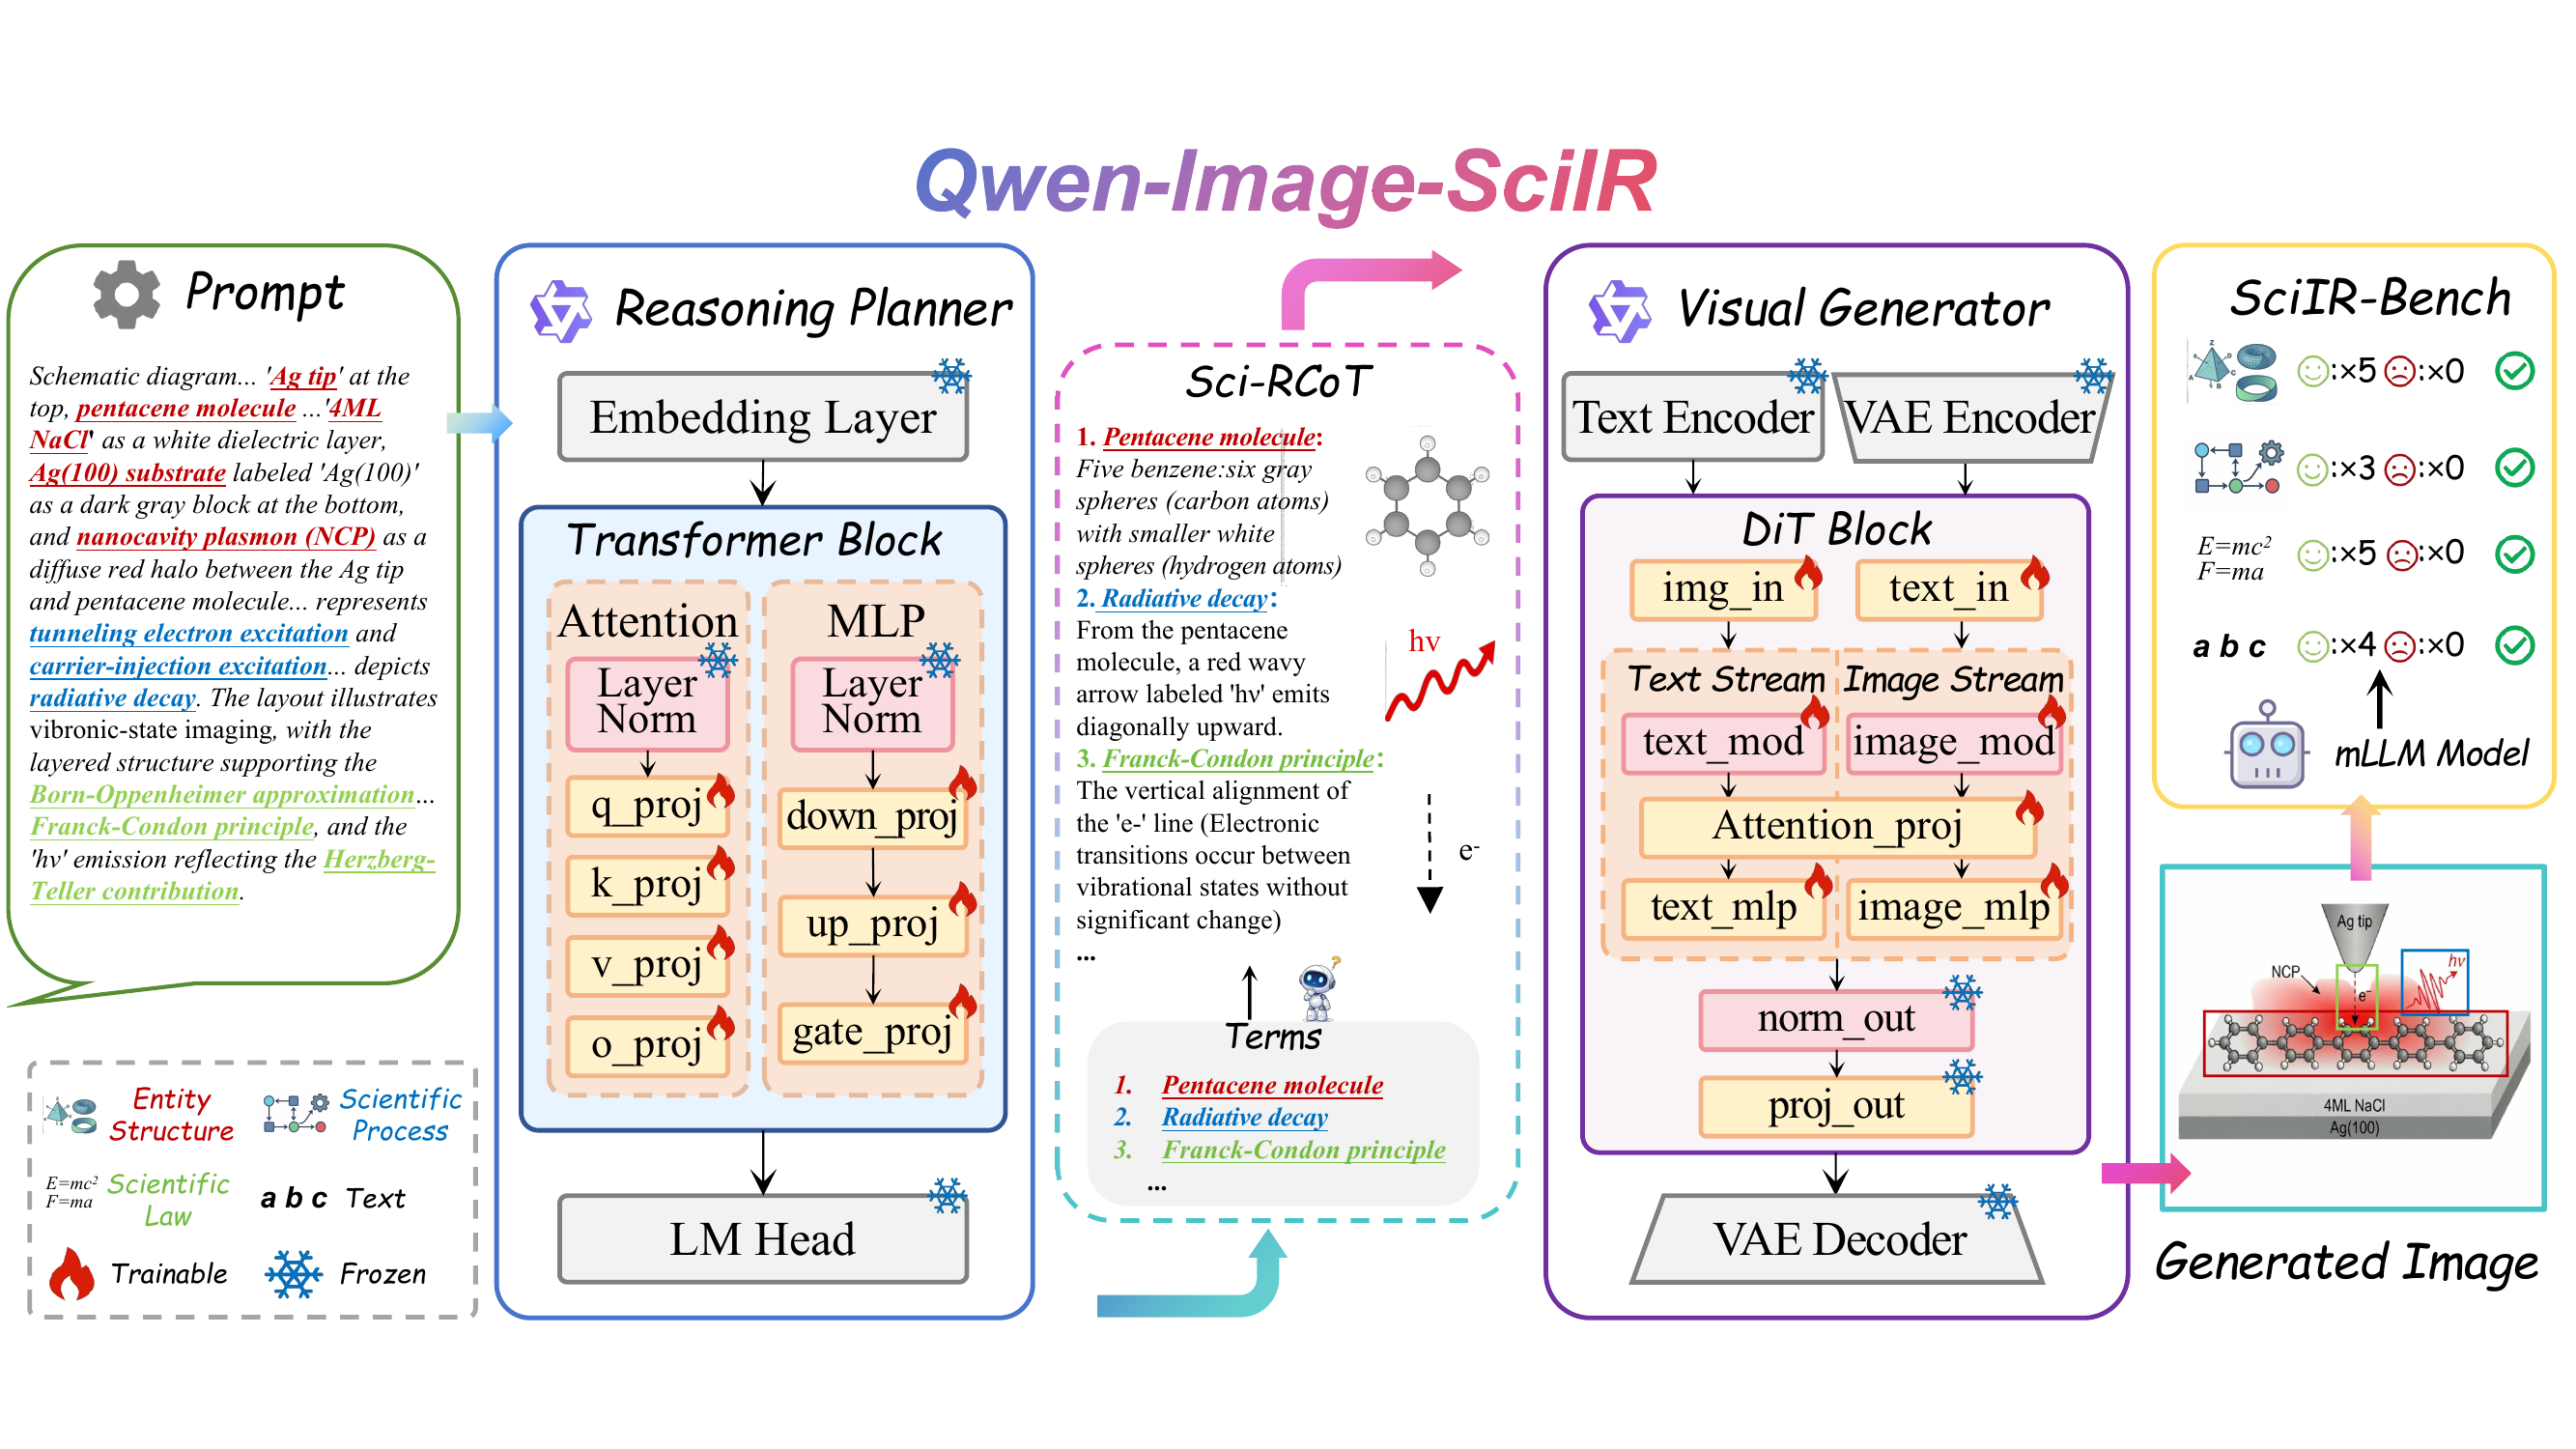
\includegraphics[width=\textwidth]{model.pdf}
    \caption{Qwen-Image-SciIR model architecture.}
    \label{fig:model}
\end{figure*}
\textbf{Implementation of Qwen-Image-SciIR.} Qwen-Image-SciIR is implemented to ensure rigorous zero-shot evaluation: we removed the 800 test instances in SciIR-Bench from the SciIR-82k corpus to avoid data leakage. As shown in Figure~\ref{fig:model}, the pipeline decouples scientific reasoning from visual synthesis via two fine-tuned modules. The first, Qwen2.5-7B-Instruct, serves as a reasoning planner and was fine-tuned on (prompt, Sci-RCoT) pairs using an all-linear LoRA configuration ($r=64, \alpha=16$). Specifically, LoRA adapters were integrated into all linear transformation layers within the Transformer blocks to maximize adaptation capacity. This module was trained with a learning rate of $1\times10^{-4}$ and a maximum context window of 2,048 tokens for one optimization step. The second, Qwen-Image-2512 as a visual generator, was fine-tuned on (Sci-RCoT, image) pairs via LoRA ($r=32$) applied to the diffusion transformer layers, with a learning rate of $1\times10^{-4}$, training resolution $1024\times1024$, and trained for one optimization step.

\textbf{Inference Protocol.} We develop a systematic inference pipeline for Qwen-Image-SciIR. Across 800 evaluation samples, encompassing both Intrinsic Reasoning (IR) and Instruction Following (IF) categories, we employ a chained generation flow. Specifically, the Reasoning Planner first infers a comprehensive Sci-RCoT from the input prompt, which is then utilized by the Visual Generator to synthesize the final image. This unified protocol ensures that the reasoning module is actively engaged for every instance, maintaining a standard reasoning-to-rendering process throughout the entire benchmark evaluation.

\subsection{Main Quantitative Results}
\cref{tab:main_results} presents the systematic evaluation of 12 T2I models across the SciIR-Bench. Our analysis reveals several key insights regarding the current landscape of scientific visual synthesis.

\textbf{Closed- \textit{vs.} Open-Source.}
Nano-Banana-pro's near-saturation performance (95\%) provides strong evidence that the task is solvable, yet a 60\% gap remains for open-source contenders. Critically, aesthetic-focused baselines like Flux-Dev fail (<10\%) on strict tracks, confirming a fundamental misalignment: current open-source training optimizes for \textit{perceptual fidelity}, sacrificing the logic essential for scientific accuracy.

\textbf{Instruction Following \textit{vs.} Intrinsic Reasoning.}
For the majority of models (\eg, GPT-Image-1, Seedream 4.5), performance under explicit Sci-RCoT prompting (IF) significantly outpaces abstract prompting (IR). For instance, FLUX.1-Kontext-Max's accuracy drops from 36\% to 13\% without dense guidance. This confirms that while they excel at executing detailed instructions, they lack internalized scientific world models to autonomously derive constraints. However, a counter-intuitive trend emerges in some open-weights models (\eg, Flux-Dev, Show-o2-7B), where IR outperforms IF. Rather than indicating superior reasoning, this highlights their deficiency in complex instruction adherence. Dense Sci-RCoT prompts overwhelm them, causing prompt overflow and attribute confusion. Thus, they paradoxically perform better on shorter abstract prompts by relying on superficial parametric memory.

\textbf{AutoRegressive \textit{vs.} Diffusion.}
Diffusion models currently maintain a distinct advantage over AutoRegressive (AR) architectures, with Qwen-Image-2512 (35\%) establishing a clear 14\% performance gap over the leading AR contender, Show-o2-7B (21\%).However, despite this architectural disparity, both paradigms share a critical vulnerability: severe failure in the Text track. With even the top models scoring merely 15\% (Diffusion) and 8\% (AR) on text generation, the results confirm a shared fundamental limitation: whether utilizing continuous denoising or discrete next-token prediction, current open-source visual generation frameworks fundamentally lack the fine-grained typographic control necessary for accurate scientific illustrating. 

\begin{figure*}[t]
    \centering
    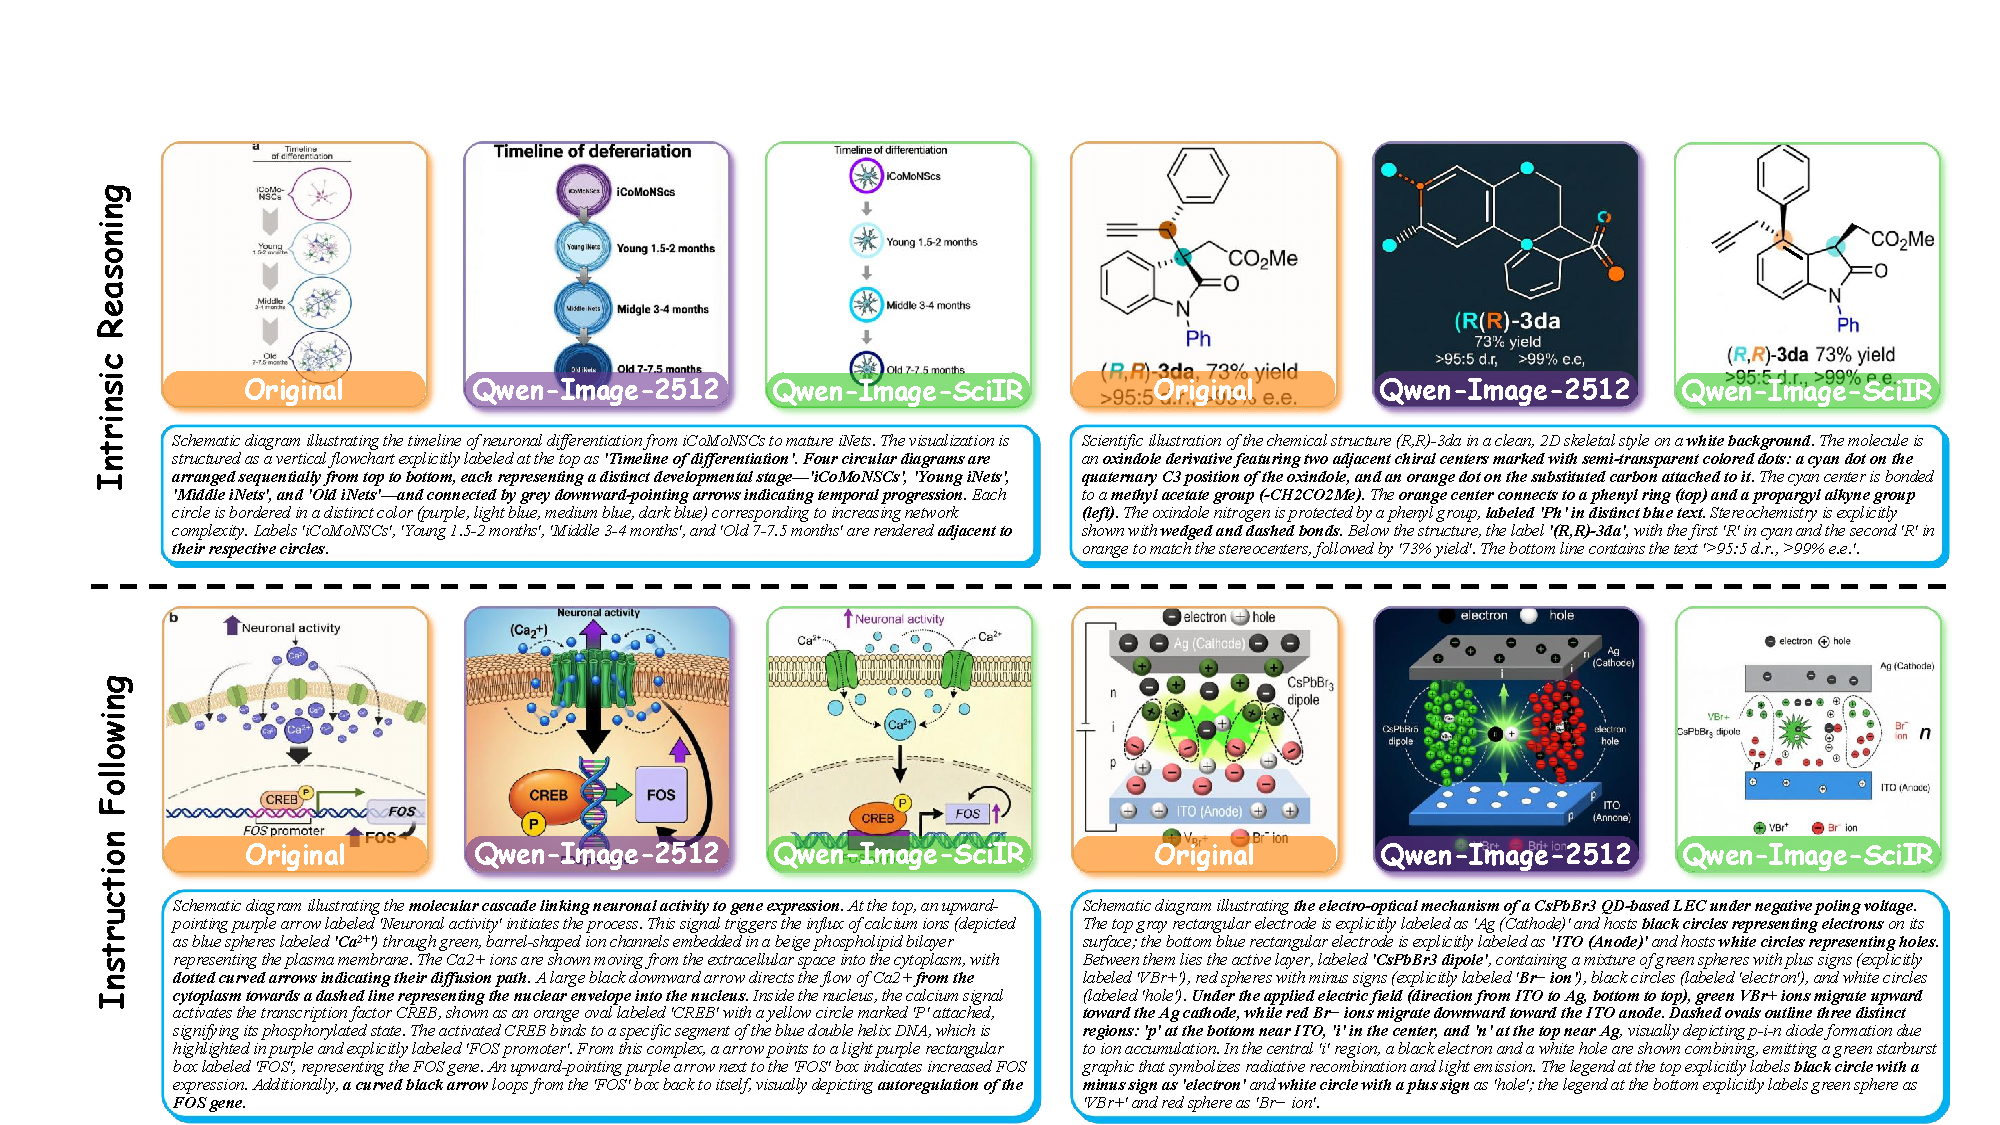
\includegraphics[width=\textwidth]{comparison.pdf}
    \caption{Qualitative comparison of generated results.}
    \label{fig:qualitative_comparison}
\end{figure*}

\textbf{Efficacy of Fine-tuning.} To validate the effectiveness of our proposed pipeline, we conduct a direct comparison between the fine-tuned Qwen-Image-SciIR and its backbone, Qwen-Image-2512. Quantitatively, \cref{tab:main_results} demonstrates a substantial performance gain, elevating the Final Score from 35\% to 43\%. This improvement is particularly pronounced in the \texttt{Scientific Process} and \texttt{Entity Structure} tracks, with increases of 16\% and 9\% respectively, indicating a robust enhancement in modeling sequential process and topological integrity.

\subsection{Qualitative Comparison}
Qualitatively, visual comparisons in \cref{fig:qualitative_comparison} reveal that Qwen-Image-SciIR shifts from a generic artistic style to a precise scientific illustration standard. We observe that the baseline Qwen-Image-2512 is prone to scientific hallucinations across three dimensions. 
The first is the \textbf{inability to correctly depict scientific processes}: it fails to visually depict the morphological progression of neuron development (top-left), relying solely on text proxies. 
The second is \textbf{morphological and structural omission}: \emph{e.g.}, in the top-right, the baseline generates non-academic redundant backgrounds and hallucinates bizarre molecular topologies that violate chemical valence rules, along with the missing nucleus in the cell cross-section (bottom-left). 
The third is the \textbf{violation of domain priors}: as seen in the bottom-right, it incorrectly grounds the charge states to their respective micro-particles (electrons, holes) and ions ($V_{\mathrm{Br}}^+$ and $\mathrm{Br}^-$). Conversely, our model effectively minimizes scientific hallucinations by explicitly integrating reasoning planning.

\subsection{Correlation Analysis}
\label{sec:correlation}
We validated our automated protocol against human expert ratings on 200 randomly sampled test cases (50 per evaluation group). Three human annotators independently performed blind scoring on these samples, with final ratings determined by averaging their scores. As shown in \cref{tab:human_correlation}, our \textit{Atomic Checklist} achieves strong alignment with domain experts ($r=0.692$), substantially outperforming the best baseline metric, VQAScore ($r=0.457$). This discrepancy suggests that embedding-based metrics may capture only superficial semantic relevance, failing to penalize subtle scientific violations (\eg, impossible topologies). In contrast, our taxonomy-grounded approach effectively detects these domain-specific hallucinations, confirming that high-fidelity scientific evaluation requires verifiable atomic constraints rather than holistic visual similarity. Implementation details are provided in Appendix G.


\begin{table}[t]
\caption{\textbf{Correlation between metrics and expert judgments.} Our Atomic Checklist shows the strongest linear and rank alignment with human experts.}
\label{tab:human_correlation}
\centering
\small
\begin{tabular}{lccc}
\toprule
\textbf{Metric} & \textbf{Pearson's $r$} $\uparrow$ & \textbf{Kendall's $\tau$} $\uparrow$ & \textbf{Spearman's $\rho$} $\uparrow$ \\
\midrule
CLIPScore\cite{hessel2021clipscore} & 0.345\textsuperscript{\tiny 4th} & 0.231\textsuperscript{\tiny 4th} & 0.315\textsuperscript{\tiny 4th} \\
VQAScore\cite{lin2024evaluating} & 0.457\textsuperscript{\tiny 2nd} & 0.342\textsuperscript{\tiny 2nd} & 0.410\textsuperscript{\tiny 2nd} \\
VIEScore\cite{ku2024viescore} & 0.412\textsuperscript{\tiny 3rd} & 0.313\textsuperscript{\tiny 3rd} & 0.389\textsuperscript{\tiny 3rd} \\
\midrule
\rowcolor{gray!20}
\textbf{Atomic Checklist (Ours)} & \textbf{0.692}\textsuperscript{\tiny 1st} & \textbf{0.596}\textsuperscript{\tiny 1st} & \textbf{0.683}\textsuperscript{\tiny 1st} \\
\bottomrule
\end{tabular}
\end{table}

% \begin{itemize}
%     \item \textbf{Structural Hallucination (Iconic Failure):} In the Entity Structure track, models frequently generate objects that are topologically incorrect despite being textured realistically. Common errors include organic molecules with impossible ring structures or lab equipment with physically disconnected components\cite{ref15}.

%     \item \textbf{Causal Inversion (Indexical Failure):} In the Scientific Process track, models often fail to respect the directionality of causality\cite{ref16}. We observed generated diagrams where arrows point from products to reactants, or where sequential experimental steps are merged into a single, incoherent state.

%     \item \textbf{Nomological Violation (Symbolic Failure):} The most critical failures occur in the Scientific Law track\cite{ref17}. Models often generate imagery that violates domain-specific constraints, such as optical diagrams where light rays bend incorrectly relative to the refractive index, or circuit diagrams that violate Kirchhoff's laws.
% \end{itemize}

\section{Conclusion}

% In this paper, we introduce \textbf{SciIR}, aimed at bridging the gap between general text-to-image models and the rigorous semantic constraints of the scientific domain. We present \textbf{SciIR-82k}, the first large-scale dataset grounded in the semiotic triad---Entity Structure, Scientific Process, and Scientific Law---alongside \textbf{SciIR-Bench}, a diagnostic evaluation benchmark. Through this framework, we uncover a substantial disparity between current open-source models and frontier proprietary systems in abstract scientific reasoning. Furthermore, we demonstrate that traditional perceptual metrics, such as CLIPScore, are insufficient for gauging the logical correctness of scientific images. Our proposed ``Atomic Checklist'' evaluation protocol exhibits high alignment with human expert judgments. We envision SciIR as a foundational platform to propel the text-to-image field beyond surface-level visual fidelity towards deep scientific logical reasoning.

SciIR proposes a principled approach to scientific image reasoning that narrows the gap between general text-to-image capabilities and the strict constraints of natural science. We release SciIR-82k, containing more than 80k high-quality science image–text pairs with traceable Sci-RCoT reasoning chains—and SciIR-Bench, a fine-grained benchmark that breaks scientific correctness into verifiable atomic checks (topology, causality, conservation, \etc). Fine-tuning on SciIR-82k yields Qwen-Image-SciIR, which raises the SciIR-Bench score from 35\% to 43\% and shows the largest gains on entity structure and scientific process tracks, demonstrating that reasoning-dense training data measurably improves scientific consistency beyond perceptual quality alone.

Despite these advances, some limitations remain. SciIR-82k is biased toward published, standardized figures and underrepresents atypical or unconventional diagrams, while SciIR-Bench emphasizes scientific correctness over visual aesthetics. Future work should broaden domain and style coverage, add multimodal and cross-lingual annotations, and investigate hybrid training and evaluation approaches—such as symbolic constraints, weak supervision, and adversarial or counterfactual checks—to further enhance the models’ ability for scientific reasoning.


% Bibliography entries for the entire Anthology, followed by custom entries
%\bibliography{anthology,custom}
% Custom bibliography entries only
\section*{Acknowledgements}
This paper is supported by the National Natural Science Foundation of China (No. 62406161)
\bibliographystyle{splncs04}
\bibliography{main}

\end{document}
